\chapter{LẬP TRÌNH VÀ THỰC NGHIỆM}

\section{Cài đặt}
Trong phần này, chúng ta sẽ trình bày môi trường phát triển và các công cụ được sử dụng trong quá trình lập trình và thực nghiệm. Python được chọn làm ngôn ngữ lập trình chính nhờ vào sự đơn giản, tính linh hoạt và khả năng hỗ trợ nhiều thư viện mạnh mẽ cho tính toán và thực nghiệm. Sau đây là các yêu cầu để cài đặt như sau:

\subsection{Windows}
\begin{enumerate}
    \item Truy cập trang web chính thức của Python tại \url{https://www.python.org/downloads/}.
    \item Tải xuống phiên bản Python 3.x mới nhất.
    \item Khi cài đặt, đánh dấu tùy chọn \textbf{Add Python to PATH} để tự động thêm Python vào biến môi trường PATH của hệ thống.
    \item Hoàn tất cài đặt bằng cách làm theo các hướng dẫn trên màn hình.
    \item Sau khi cài đặt, mở \index{Command Prompt} (CMD) và kiểm tra bằng cách gõ lệnh:
    \begin{verbatim}
    python --version
    \end{verbatim}
    Lệnh này sẽ trả về phiên bản Python đã cài đặt nếu quá trình cài đặt thành công.
\end{enumerate}

\subsection{MacOS}
\begin{enumerate}
    \item Mở Terminal và cài đặt Homebrew (nếu chưa cài đặt) bằng lệnh:
    \begin{verbatim}
    /bin/bash -c "$(curl -fsSL https://raw.githubusercontent.com/Homebrew/install/HEAD/install.sh)"
    \end{verbatim}
    \item Sau khi cài đặt Homebrew, cài đặt Python bằng lệnh:
    \begin{verbatim}
    brew install python
    \end{verbatim}
    \item Kiểm tra phiên bản Python đã cài đặt bằng lệnh:
    \begin{verbatim}
    python3 --version
    \end{verbatim}
\end{enumerate}

\subsection{Linux (Ubuntu)}
\begin{enumerate}
    \item Mở \index{Terminal} và cập nhật danh sách gói bằng lệnh:
    \begin{verbatim}
    sudo apt update
    \end{verbatim}
    \item Cài đặt Python 3 bằng lệnh:
    \begin{verbatim}
    sudo apt install python3
    \end{verbatim}
    \item Kiểm tra phiên bản Python đã cài đặt:
    \begin{verbatim}
    python3 --version
    \end{verbatim}
\end{enumerate}

\subsection{Cài đặt công cụ quản lý gói (pip)}
\texttt{pip} là công cụ quản lý gói của Python, dùng để cài đặt các thư viện và gói mở rộng. Sau khi cài đặt Python, bạn có thể kiểm tra phiên bản \texttt{pip} bằng lệnh:
\begin{verbatim}
pip --version
\end{verbatim}
Nếu chưa cài đặt, bạn có thể cài đặt \texttt{pip} theo các bước sau:

\subsubsection{Cài đặt \texttt{pip} trên Windows/MacOS/Linux}
\begin{verbatim}
python -m ensurepip --upgrade
\end{verbatim}

\subsection{Cài đặt các gói thư viện cần thiết}
Các gói thư viện cần thiết sẽ được lưu trữ trong tệp requirements.txt kèm theo với mã nguồn. Để cài đặt tất cả các thư viện từ file \texttt{requirements.txt}, bạn sử dụng lệnh:
\begin{verbatim}
pip install -r requirements.txt
\end{verbatim}

% \section{Kết quả}

% \section{Hướng dẫn đánh giá}
% Toàn bộ mã nguồn và tệp đánh giá thuật toán chúng tôi để tại đây: <link>. Sau khi tải về, hãy thực hiện theo các lệnh dưới đây:


\section{Thử nghiệm và đánh giá}


\subsection{Thử nghiệm với các ví dụ nhỏ}


\begin{figure}[H]
    \centering
    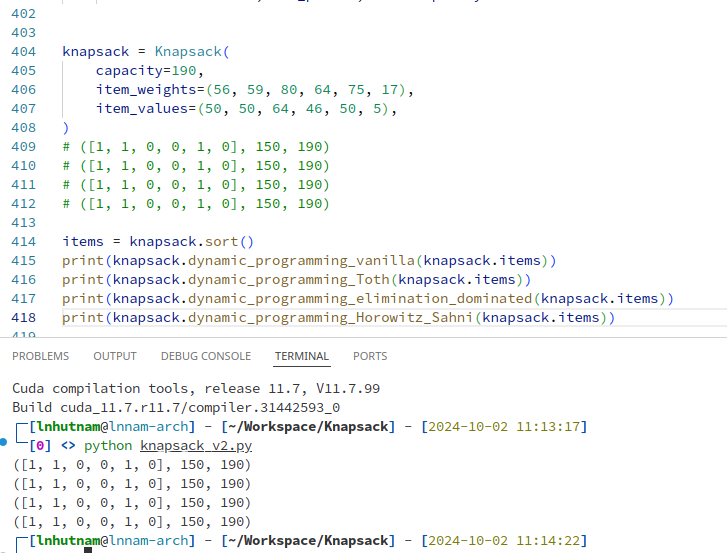
\includegraphics[width=1\columnwidth]{figures/vd.png}
    \caption{Thí nghiệm Ví dụ 1.}
    \label{fig:test1}
\end{figure}

\begin{figure}[H]
    \centering
    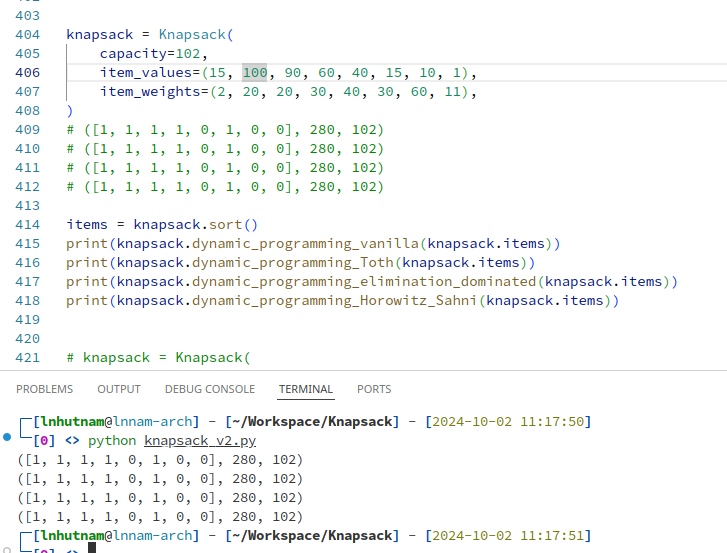
\includegraphics[width=1\columnwidth]{figures/vd2.png}
    \caption{Thí nghiệm Ví dụ 2.}
    \label{fig:test1}
\end{figure}


\subsection{Đánh giá thời gian và độ phức tạp bộ nhớ thực thi}
    Do quá trình thực thi các thuật toán ``dynamic\_programming\_Horowitz\_Sahni`` và ``dynamic\_programming\_elimination\_dominated``. tốn rất nhiều tài nguyên tính toán, trong khi tài nguyên không đáp ứng đủ. Vì vậy, trong phần đánh giá này, chúng tôi sẽ không đánh giá cho kết quả hai thuật toán trên.

    Data đánh giá bao gồm 3 bộ dữ liệu là \textbf{00Uncorrelated}, \textbf{02StronglyCorrelated} và \textbf{12Circle}. Mỗi bộ gồm 4 tập tin chứa thông tin của bài toán Knapsack với số lượng đồ vật lần lượt là 50 và 100; dung lượng túi tăng dần.

 \subsubsection{Phức tạp thời gian}

\begin{table}[H]
\centering
    \begin{tabular}{|c|c|}
    \hline
    \textbf{Thuật toán} & \textbf{Thời gian (ms)}           \\ \hline
    greedy\_binary      & 0.06644        \\ \hline
    greedy             & 0.05246         \\ \hline
    dynamic\_programming\_vanilla             & 7956.2574         \\ \hline
    dynamic\_programming\_Toth             & 1407.7398         \\ \hline
    \end{tabular}
    \caption{Thời gian chạy của các thuật toán}
\end{table}


 \subsubsection{Phức tạp bộ nhớ}

 \begin{table}[H]
\centering
    \begin{tabular}{|c|c|}
    \hline
    \textbf{Thuật toán} & \textbf{RAM (MB)}           \\ \hline
    greedy\_binary      & 0.00016        \\ \hline
    greedy             & 0.00130        \\ \hline
    dynamic\_programming\_vanilla             & 4.7073         \\ \hline
    dynamic\_programming\_Toth             & 1.0294         \\ \hline
    \end{tabular}
    \caption{RAM sử dụng của các thuật toán}
\end{table}

\textbf{Nhận xét:} Với họ thuật toán Greedy sẽ cho kết quả thời gian và sử dụng RAM tốt hơn so với hai thuật toán còn lại, tuy nhiên như đã trình bày, hai thuật toán này không cho kết quả tối ưu, chúng tôi đưa vào đây để lấy làm căn cứ so sánh. Trong khi đó, thuật toán quy hoạch động Toth cho kết quả tốt trên cả thời gian và độ phức tạp bộ nhớ (tương ứng là 6x và 3x). Điều này phù hợp với lý thuyết chúng tôi đã trình bày ở chương trước.

\subsection{Hướng dẫn chạy đánh giá}
\begin{itemize}
    \item [1.] Chạy đánh giá trên tập dữ liệu
    \begin{verbatim}
    python3 knapsack.py --data [input-data]
                        --output [output-save] --mode eval
    \end{verbatim}

    Ví dụ:
    \begin{verbatim}
    python3 knapsack.py --data kplib --output output --mode eval
    \end{verbatim}

    \item [2.] Chạy test kết quả:
    \begin{verbatim}
    python3 knapsack.py --mode infer
    \end{verbatim}

    - Màn hình hỏi: \textbf{input capacity:}, nhập dung lượng túi, ví dụ: 10

    - Màn hình hỏi: \textbf{input weights, separated by `,`:}, nhập khối lượng từng vật phân cách bởi dấu ``,``, ví dụ: 5,7,3

    - Màn hình hỏi: \textbf{input values, separated by `,`:}, nhập giá trị từng vật phân cách bởi dấu ``,``, ví dụ: 5,15,6.

    - Kết quả:
    \begin{verbatim}
    input capacity:
    10          
    input weights, separated by `,`:
    5,7,3
    input values,  separated by `,`:
    5,15,6
    greedy:
    solution: (0, 1, 1)
    value: 21
    greedy_binary:
    solution: (0, 1, 1)
    value: 21
    dynamic_programming_vanilla:
    solution: [0, 1, 1]
    value: 21
    dynamic_programming_Toth:
    solution: [0, 1, 1]
    value: 21
    dynamic_programming_Horowitz_Sahni:
    solution: [0, 1, 1]
    value: 21
    dynamic_programming_elimination_dominated:
    solution: [0, 1, 1]
    value: 21
    \end{verbatim}
    
\end{itemize}